\documentclass[letterpaper, twocolumn, 9pt]{article}
\usepackage[table]{xcolor}

\usepackage[margin=0.75in, columnsep = 1.5cm]{geometry}
\usepackage[parfill]{parskip} % Allows paragraphs to begin with an empty line rather than an indent
\usepackage{enumerate}
\usepackage{wallpaper}
\usepackage{fancyhdr}
\usepackage{texshade}
\usepackage{amsmath}
\usepackage{mathtools}
\usepackage[colorlinks=FALSE]{hyperref}
\usepackage{enumitem}
\usepackage[numbers, square]{natbib}
%\usepackage{multirow}
\usepackage[font=small, width=.95\columnwidth]{caption}
\usepackage{subcaption} % for subfiguress
\usepackage{soul} % for highlighting text
\newcommand{\hlc}[2][yellow]{ {\sethlcolor{#1} \hl{#2}} } % for having more than one highlighter color: hlc[green]{some text}

%%%%% CODE DISPLAY
\usepackage{listings} % for code display; see https://en.wikibooks.org/wiki/LaTeX/Source_Code_Listings for more formatting options
\definecolor{lightlightgray}{rgb}{0.95,0.95,0.95} 
\lstset{
    language=bash,
    tabsize=2,
    breaklines=true,
    commentstyle=\color{blue},
    basicstyle=\ttfamily\small,
    keywordstyle=\color{magenta},
    backgroundcolor=\color{lightlightgray},
    morecomment=[l][\color{darkgreen}]{\#\$},
    morekeywords={awk, chmod, configure, cp, cut, grep, head, ls, make, mkdir, montage, rm, samtools, sed, slchoose, tar, unzip, wc, wget, xargs},
    deletekeywords={source},
    showstringspaces=false,
    showspaces=false,
    showtabs=false,
    breaklines=true,
    captionpos=b,
    frameround=tttt, % rounds the corners
    frame=trbl,      % prints a frame. (uppercase makes a double line frame)
    xleftmargin=.02\textwidth, xrightmargin=.02\textwidth,
    numbers=left, numberstyle=\tiny, numbersep=5pt}

\newcommand{\bangbox}[1] {
\begin{center}
  \fcolorbox{MidnightBlue}{CornflowerBlue!20}{ % this makes 20% Blue, 80% white
    \begin{minipage}{0.05\linewidth}
      \includegraphics[width=\textwidth]{figures/exclamationmark}
    \end{minipage}
    \begin{minipage}{0.90\linewidth}
      #1
    \end{minipage}
  }
\end{center}
}

\setlength{\unitlength}{2em} % for the picture environment for flow_errbs
\setlength{\columnseprule}{.5pt} % for the vertical line

% resetting the footnote format
\makeatletter
\newlength{\fnBreite}
\renewcommand{\@makefntext}[1]{%
  \settowidth{\fnBreite}{\footnotesize\@thefnmark.i}
  \protect\footnotesize\upshape%
  \setlength{\@tempdima}{\columnwidth}\addtolength{\@tempdima}{-\fnBreite}%
  \makebox[\fnBreite][l]{\@thefnmark.\phantom{}}%
  \parbox[t]{\@tempdima}{\everypar{\hspace*{1em}}\hspace*{-1em}\upshape#1}}
\makeatother
%%%%%%

\title{PCP: An R-based application for visualization data from protein correlation profiling}
\date{revised \today}
\author{Prepared for Noah Dephoure, Weill Cornell Medical College\\ 
by the Applied Bioinformatics Core (ABC), Weill Cornell Medical College}

\pagestyle{fancy}
%\fancyhf{}
%\fancyhead[C]{\textit{PCP}}
\fancyhead{}
\fancyhead[CO, CE]{\leftmark}
%\fancyhead[RE]{\rightmark}
\cfoot{\thepage}

\usepackage{titlesec}
\setcounter{secnumdepth}{4}

%\titleformat{\paragraph}
%{\normalfont\normalsize\bfseries}{\theparagraph}{1em}{}
%\titlespacing*{\paragraph}
%{0pt}{3.25ex plus 1ex minus .2ex}{1.5ex plus .2ex}


\ThisULCornerWallPaper{1}{../../wcmc_abc_logo.pdf}

%%%%%%%%%%%%%%%%%%%%%%%%%%%%%%%%%%%%%%%%%%%%%%%%%%%%%%%%%%%%%%%%%%%%%%%%%%%%%%%%%%%%%
\begin{document}
\onecolumn
\frenchspacing 
\maketitle

\tableofcontents
%\listoffigures
%\listoftables 
\clearpage

\twocolumn
%============================
\section{Installation and updating}
%============================

The routine for installing and updating the package is the same (with the exception of the \texttt{devtools} installation, which must be done only once).

\begin{enumerate}
\item Open RStudio.
\item{ In the \textsf{Console} section of RStudio, type:
\begin{lstlisting}
# install helper package (must be done only once!)
> install.packages("devtools")

# download the source of the package and install it
# note that the version number will change depending on the update
# you can check which version is appropriate at http://chagall.med.cornell.edu/deplab-pcp/
> devtools::install_url(url = "http://chagall.med.cornell.edu/deplab-pcp/DepLab_0.1.1.9000.tar.gz")

# attach the package to your current R environment
> library(DepLab)

# start the interactive app
> runPCP()
\end{lstlisting}}
\end{enumerate}


%============================
\section{Start}
%============================

If you have installed the most recent version of the package and you just want to continue using the app, all you need to do is:

\begin{enumerate}
\item Open RStudio.
%\item{Move to the folder where the app is stored.
%\centering{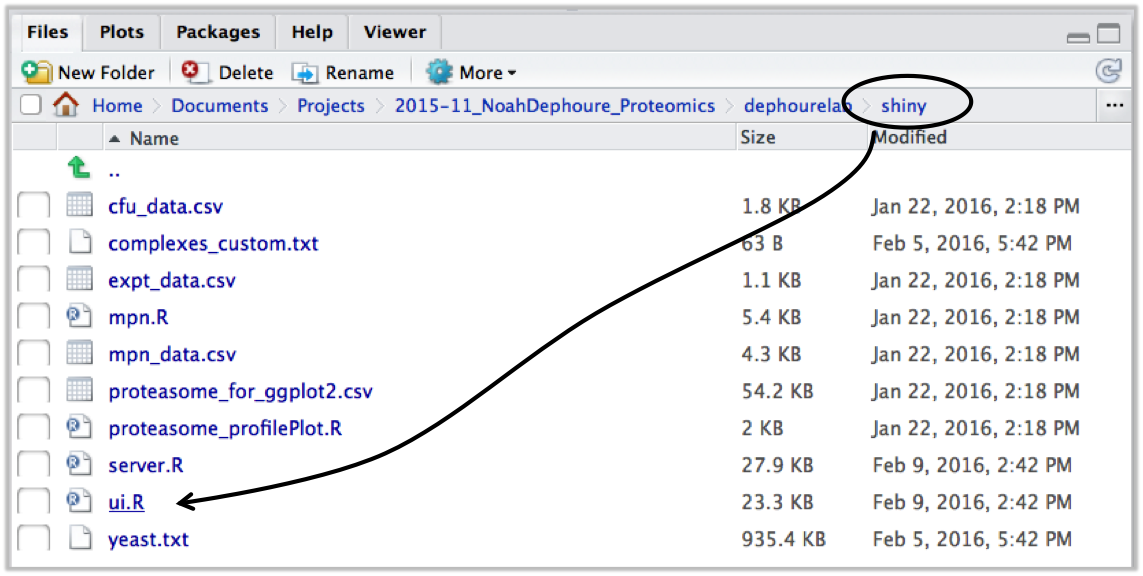
\includegraphics[width=.98\columnwidth]{figures/ss_startApp.png}}}
%\item{Open the file \texttt{ui.R}, then click on the \textsf{``Run App"} symbol that will appear in the text editor field of RStudio.
%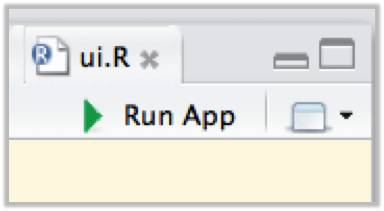
\includegraphics[scale=.7]{figures/ss_startApp02.png}
%	This will open the application.}
\item{ In the \textsf{Console} section of RStudio, type:
\begin{lstlisting}
> library(DepLab)
> runPCP()
\end{lstlisting}

This will start the application in a new window.}
\end{enumerate}

%============================
\section{Using the app - overview}
%============================

There are three main parts to the app:

\begin{tabular}{p{2.5cm}p{4.8cm}}
\hline
  \textbf{Data Import} & specify the file that contains the results of a protein correlation profiling experiment and add it to the data base \\
  \hline
  \textbf{Visualization} & generate plots for all values that \texttt{MaxQuant} reported per eluted fraction \\
  \hline
  \textbf{Tables} & explore the values underlying a specific plot in tabular format \\
  \hline  
\end{tabular}

While the \textsf{Data import} panel will always be shown at the start of the app, you can skip right to the visualization or tables part without uploading a new file. You will, however, need to make sure you have selected the correct data base.


%============================
\section{Data import}
%============================
\label{sec:dataup}

The app allows for the import of a table of proteins that were identified during a protein correlation profiling experiment.
Every file that is uploaded will be stored in a relational \texttt{sqlite} database.
This allows for storing (and retrieval) of multiple data files in a consistent manner including customized metadata entries, such as information about the specific experiment, the date of data acquistion etc. (see Section~\ref{ref:metadata}).
This also means that the database will grow over time as more and more files are added.

\bangbox{The data base should be regularly backed up.}

Once you start the app, you will be shown the path to the database that you used during your last session.
You will also see the experiment IDs of the data sets that were previously stored.
You can change the path to the data base via the \textsf{Select database} button, but we strongly recommend to keep all the data in \textit{one} database rather than scattering information from different experiments into different databases.

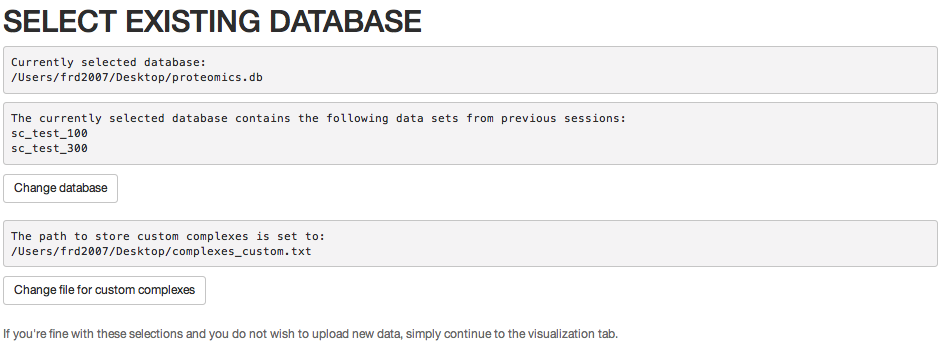
\includegraphics[width=.98\columnwidth,trim={0 0 17cm 0},clip]{figures/ss_selectDB.png}

In addition, you can check and change the path to the text file where the custom-defined complexes are stored.

To upload a file, the current workflow is as follows:
\begin{enumerate}
\item{Select the \textsf{``Data Import"} tab.


\includegraphics[width=.75\columnwidth]{figures/ss_appOverview.png}}

\item{ Click on \textsf{``Choose File"} and navigate to the \texttt{MaxQuant} output file.
Currently, the app accepts the \texttt{proteinGroups*.txt} output of \texttt{MaxQuant} \citep{MQ2008, MQ2012}.
For each protein group, only the founder protein will be extracted.
% In shotgun proteomics experiments, it is common to obtain inferred protein groups rather than unambiguously identified proteins because peptides may match more than one protein (including splice isoforms and paralogs). MaxQuant lists the founder protein of each group first; subsequent proteins may map to only a subset of these peptides. A new group is generated only when a peptide cannot be sorted into any of the existing protein groups. This algorithm will therefore always create the shortest possible list of protein groups capapble of explaining all peptide identifications. \citep{MQ2012}
 There should be a bar indicating that the upload was successful.

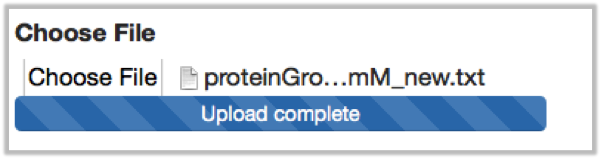
\includegraphics[scale=.6]{figures/ss_dataUpload.png}}
\item Specify a \textit{unique experimental ID} which will help you identify the experiment later on. 
\item Select the \textit{organism} from which the samples of that particular experiment originated from.
\item If you know the UniProt ID of the protein you have used as a \textit{standard} for that particular experiment, indicate that in the field below the experimental ID. If you do not specify a UniProt ID, the default is to retrieve the values related to trypsin (from pig) in that data set.
\item Fill out all the relevant metadata connected to that particular experiment (for details, see Section~\ref{sec:metadata}).
\item{ Click \textsf{``Save"}. Since this will load all the entries from the \texttt{MaxQuant} output into the database, this may take a while. Once the updating of the database has succeeded, you will see a corresponding message.}
\end{enumerate}

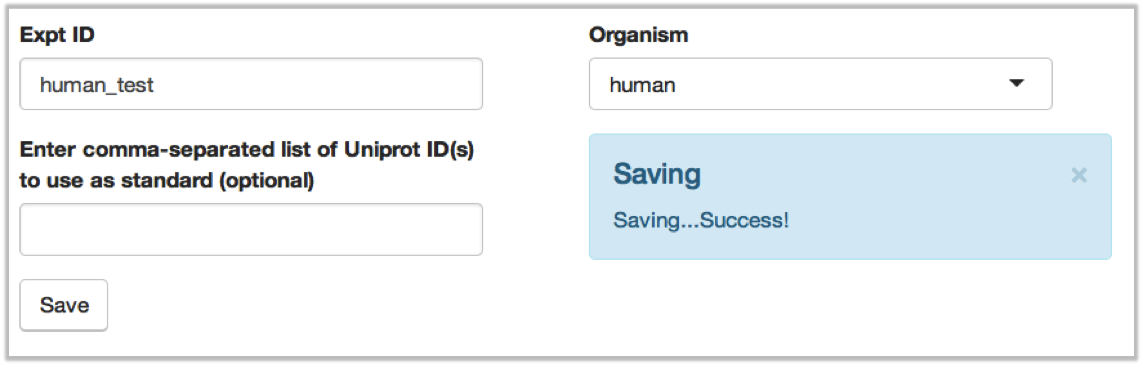
\includegraphics[width=\columnwidth]{figures/ss_dataUpload02.png}

\bangbox{It is not possible to upload a file with a previously used experimental ID.
Metadata, however, can be updated and corrected after upload (see Section~\ref{sec:edit}).}

%---------------------------------------
\subsection{Metadata}\label{sec:metadata}
%---------------------------------------

As of \texttt{DepLab v0.1.1}, you will be required to provide some basic metadata, i.e., additional information about the experiment for which you are uploading the data.
The mandatory entries include the name of the experimenter, the genotype, harvest data, lysis method etc.

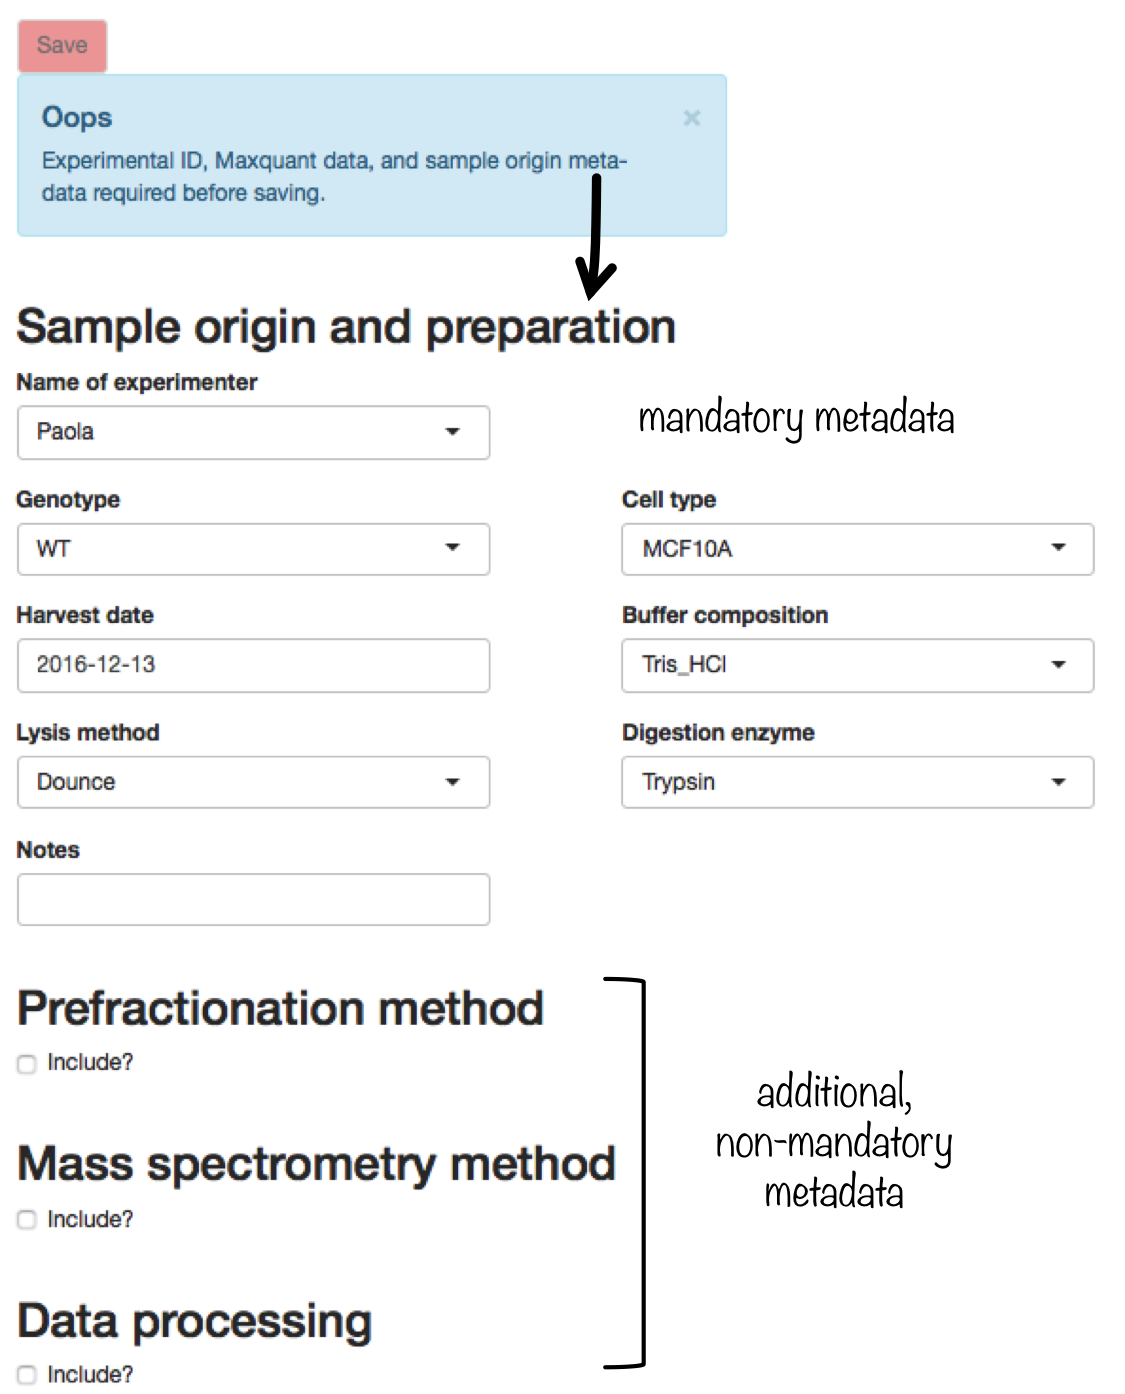
\includegraphics[width=\columnwidth]{figures/ss_dataUpload03.png}


Additional types of metadata can be added:
\begin{itemize}
\item \textsf{Prefraction method} captures information such as column ID, amount of loaded protein, sample volume, time per and number of fractions. 
\item \textsf{Mass spectrometry method} expects information about the Instrument ID, the run date (default will be the current day) and the length of the method.
\item \textsf{Data processing} lets you keep track of basic software settings that were used for the processing of the spectra, such as the search and filtering algorithms.
\end{itemize}

\bangbox{If you need more pre-defined entries -- e.g., for the name of the experimenter -- get in touch with us (\url{frd2007@med.cornell.edu}).}

You can check the metadata entered for the experiments within the selected database in the \textsf{Database} section (\textsf{DB Viewer}).


\includegraphics[width=\columnwidth]{figures/ss_appOverview04.png}
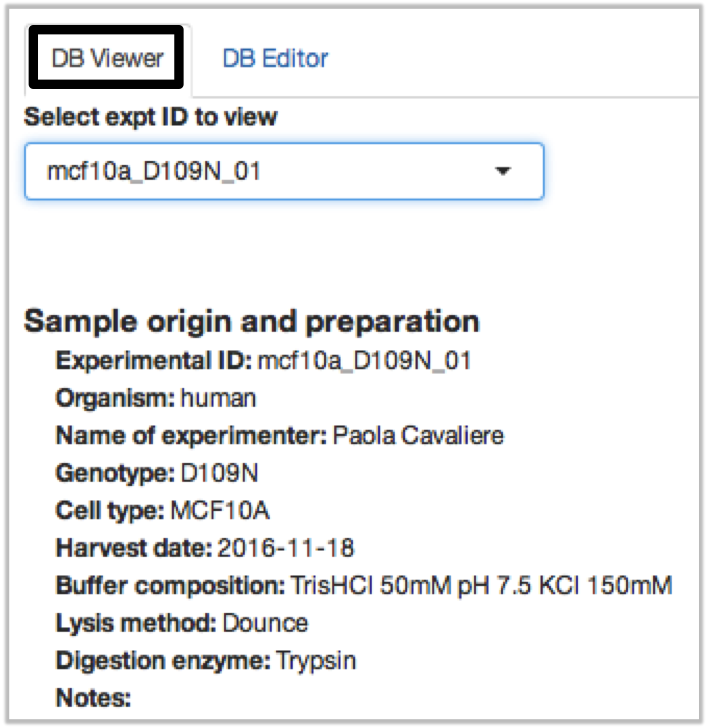
\includegraphics[width=.8\columnwidth]{figures/ss_dbviewer.png}

%.......................................
\subsubsection{Editing the metadata already stored in the data base}\label{sec:edit}
%.......................................

To edit the metadata related to experimental data within the selected database, go to the \textsf{DB Editor} in the \textsf{Database} section.
Just select the experiment ID of the experiment for which you would like to change the metadata.
Then add the respective changes and hit \textsf{"Save changes"}.


\includegraphics[width=\columnwidth]{figures/ss_appOverview04.png}
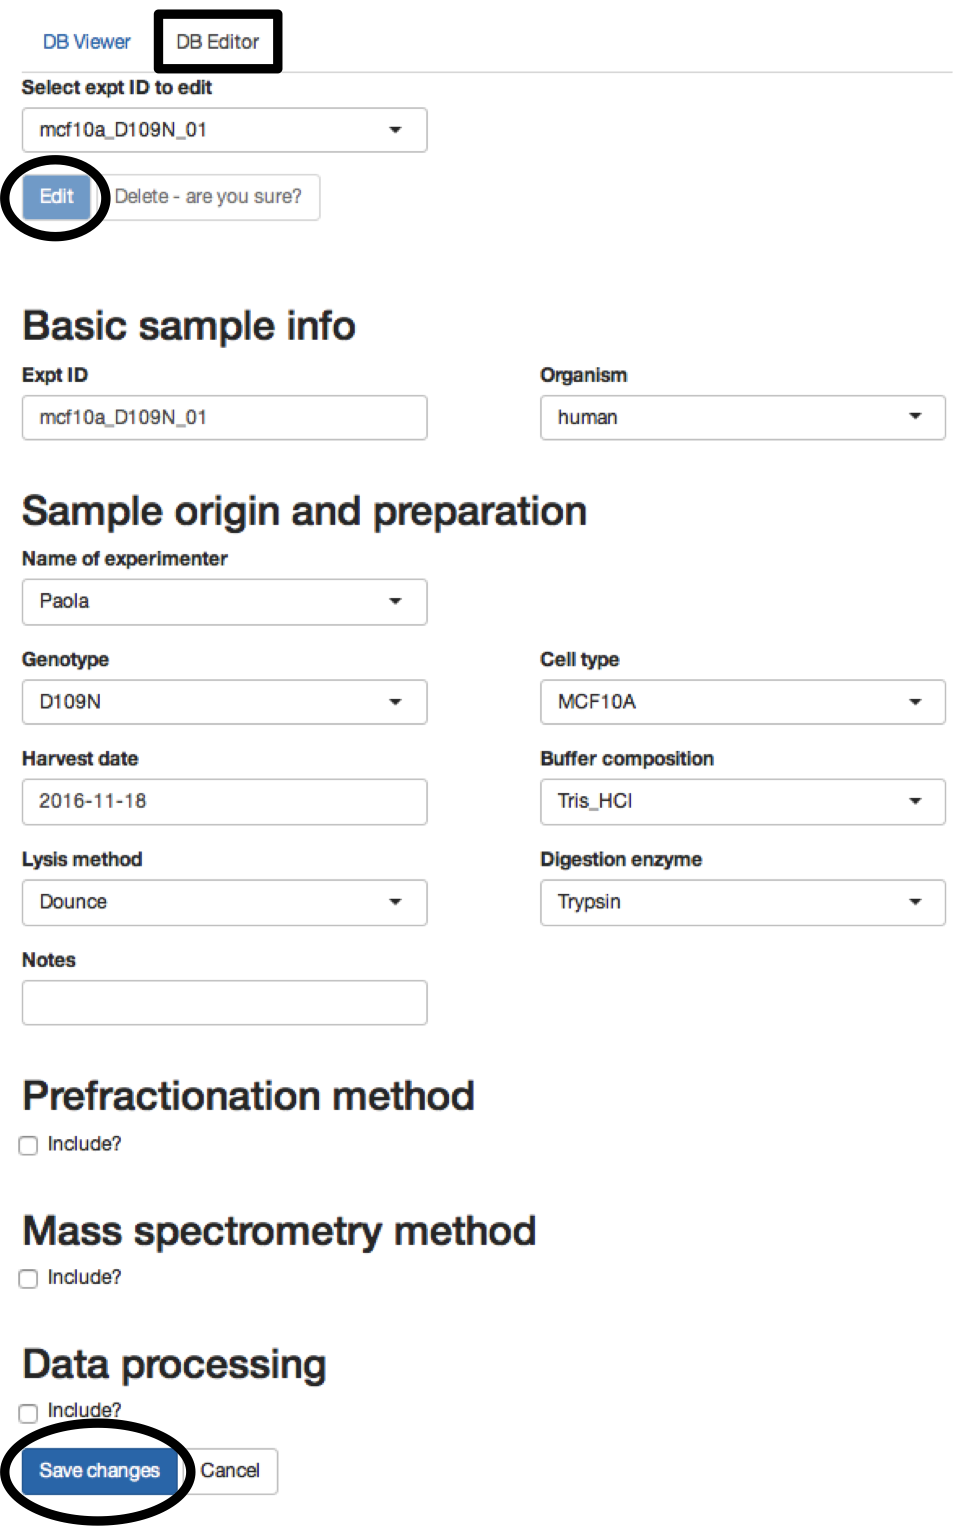
\includegraphics[width=\columnwidth, trim={0 20cm 5cm 0},clip]{figures/ss_dbeditor.png}

You can also delete all information related to an entire experiment by clicking the\textsf{Delete} button.

%============================
\section{Visualizing protein profiles}
%============================


\includegraphics[scale=.5]{figures/ss_appOverview02.png}

There are three kinds of plots that can currently be generated to visualize the fraction-wise protein profiles:

\begin{enumerate}
\item \textbf{Summary plot:} Depicting the sums of values for all protein groups per fraction.
\item \textbf{Individual proteins:} Tracking the measured values across all fraction for individual proteins and complexes.
\item \textbf{Spike-in:} Tracking the values for the protein spike-in controls across the fractions.
\end{enumerate}

The general steps to obtain a plot are very similar for all three types:

\begin{enumerate}[noitemsep]
\item Select the \textit{type of plot} that you would like to generate.
\item{Select \textit{one or more experiments}. The field \textsf{``Select expt ID"} will contain all experimental IDs stored in the database. You can choose by scrolling through the list or typing the specific ID.

\centering{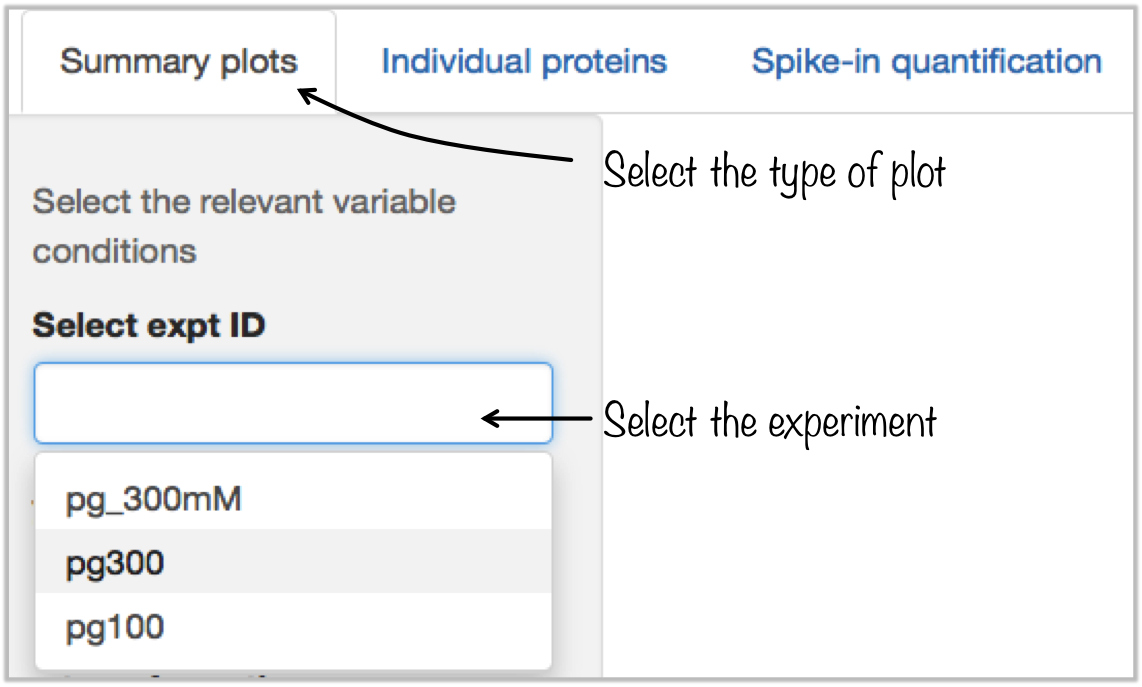
\includegraphics[scale=.35]{figures/ss_plotsOverview.png}}}
\end{enumerate}

Once you select the experiment ID, a plot will immediately be generated using default settings that currently include to use the raw intensity for the $y$ variable and to make a separate plot for each selected experiment ID.

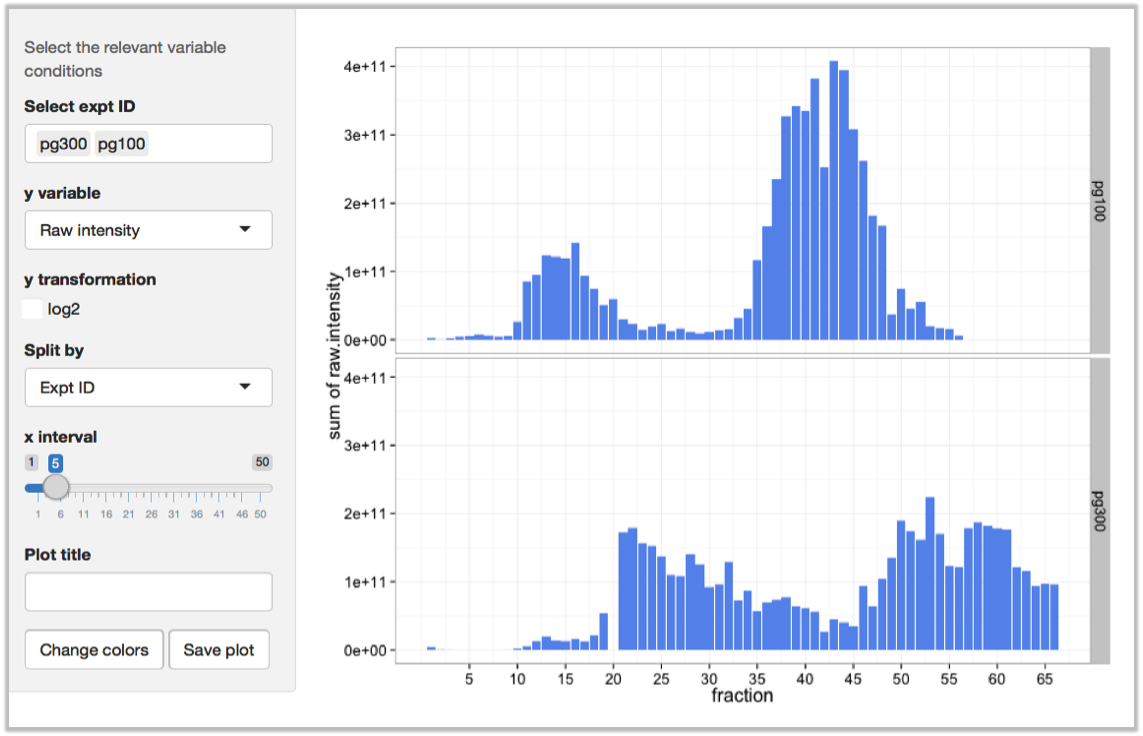
\includegraphics[scale=.4]{figures/ss_plotsOverview02.png}

All images can be saved as pdf or png files (\textsf{``Save plot"}).

%---------------------------------------
\subsection{Interacting with the protein profiles}
%---------------------------------------

The plots can be customized in various ways.
Every change will immediately refresh the image.

The \textit{size of the plot} is connected to the size of the app's display.
If you reduce the size of the app's window, the plot will be adjusted accordingly.

To \textit{zoom} into certain fractions, simply use the mouse to draw a rectangle around the region of interest.
Then double-click into the light blue blox.

\begin{center}
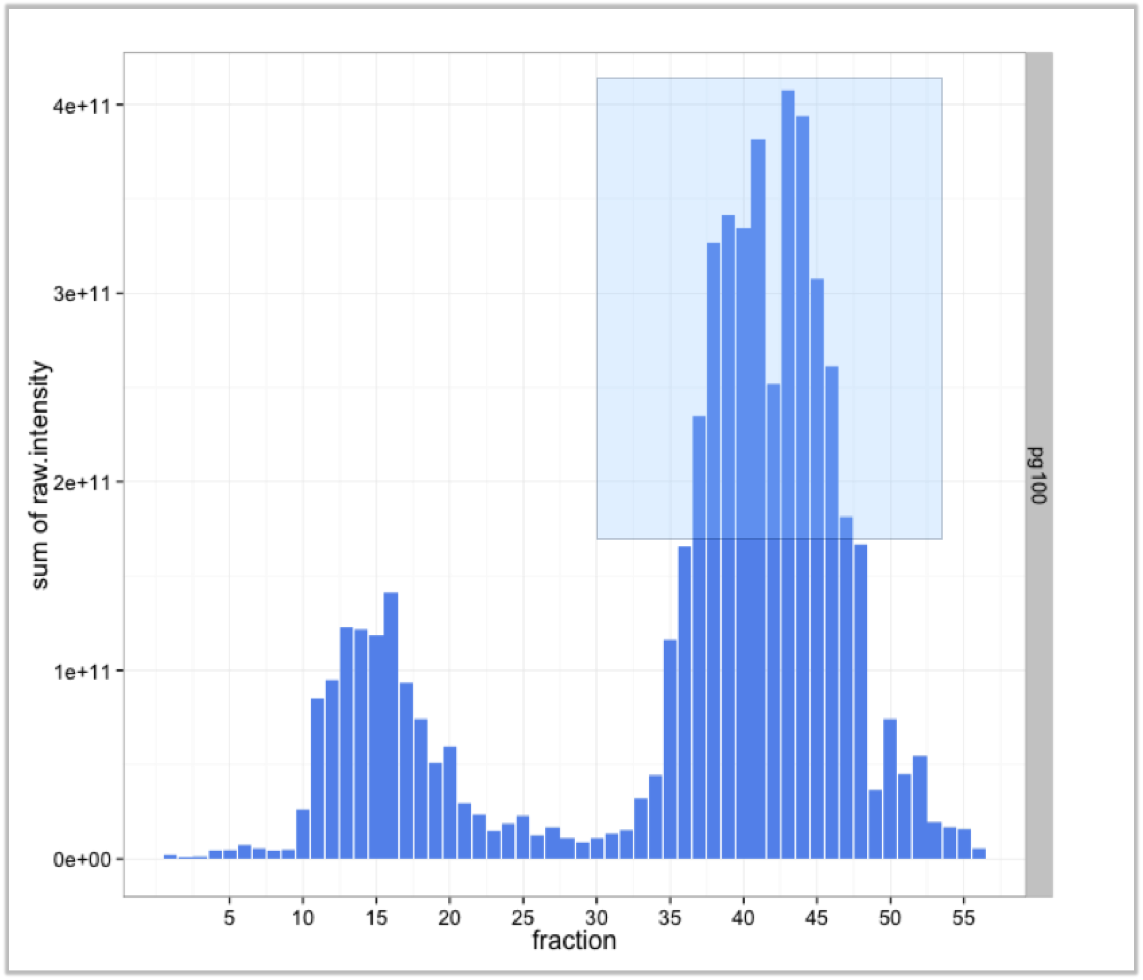
\includegraphics[width=.9\columnwidth]{figures/ss_plotCustomizing01.png}
\end{center}

To zoom out to the original scale, double click anywhere within the image.

To \textit{retrieve basic information} from UniProt for each depicted molecule, click on the respective link underneath each plot (scroll down if you don't see it immediately).
Since the download from UniProt takes some time, this list is not automatically updated if you change the selection of proteins.
You will have to refresh that list manually.
If you click on the individual UniProt IDs within the result table, the corresponding web site will be opened in your Internet browser.

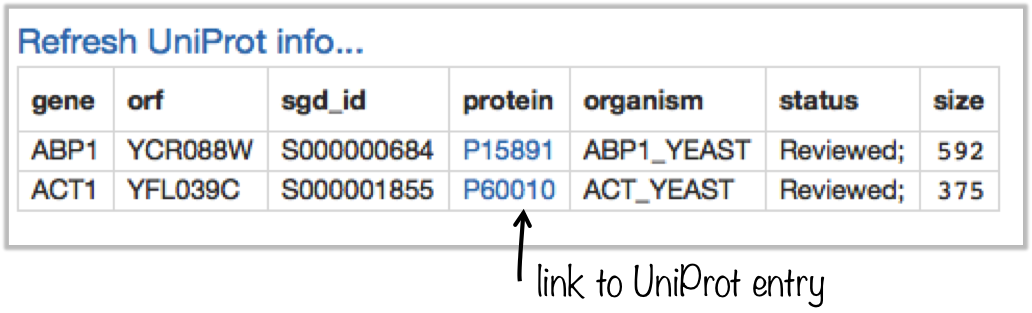
\includegraphics[scale=.4]{figures/ss_uniProtInfo01.png}

%---------------------------------------
\subsection{Values for display}
%---------------------------------------

The following measurements are available for all three kinds of plots (\textsf{``y variable"}):

\begin{itemize}[noitemsep]
\item Raw intensity
\item LFQ intensity
\item MS count
\item Peptides count % high peptide counts indiciate ambiguity
\item Unique peptides only
\item Razor and unique peptides % razor peptides are not unambiguous; they are assigned to the protein group with the highest number of total peptide identifications ("Occam's razor")
\item Sequence coverage % percentage of coverage of the leading protein within a group
\end{itemize}

These are all the numerical values that \texttt{MaxQuant} supplies per fraction.

For the \emph{individual protein plots}, these numerical values can be modified to improve the effectiveness of the visualization.

\begin{center}
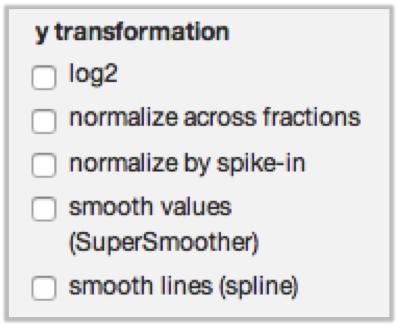
\includegraphics[scale = .5]{figures/ss_ytrafo.png}
\end{center}

\begin{itemize}\label{sec:norm}
\item \textsf{Normalize across fractions:} Each measured value, $m_f$, is normalized so that proteins with equal measurements in each fraction, $f$, have a normalized value of 1 per fraction: $m_{norm} = \frac{m_f\, \times \, F}{\sum\limits_{f=1}^{F} m}$.
\item \textsf{Spike-in control:} Each measured value, $m_f$, is normalized to the corresponding value, $s_f$, of the spiked-in protein: $m_{norm} = \frac{m_f}{s_f}$.
\item \textsf{Smooth values (SuperSmoother):} This will apply Friedman's SuperSmoother, which is a sophisticated moving average method \citep{Friedman1984}.
\item \textsf{Smooth lines (spline)}: This applies a function that interpolates the numerical values using polynomial functions \citep{Blanc1995}.
\end{itemize} 

%---------------------------------------
\subsection{Customizing the colors}
%---------------------------------------

You can change the color scheme via the button \textsf{``Change colors"}.
Once you click on it, a separate window will appear which will allow you to change the type of color scheme (qualitative, sequential, diverging), choose the colors, manipulate hue\footnote{Hue: The degrees on the RGB color wheel where Red = 0, Green = 120, Blue = 240.}, chroma\footnote{Chroma: The saturation of the hue indicated with values 0 (black) to 255.}, luminance\footnote{Luminance: Perceived brightness of a color; depends on the hue as well as the saturation.} and power, and specify the numbers of colors that will be used.
\begin{center}
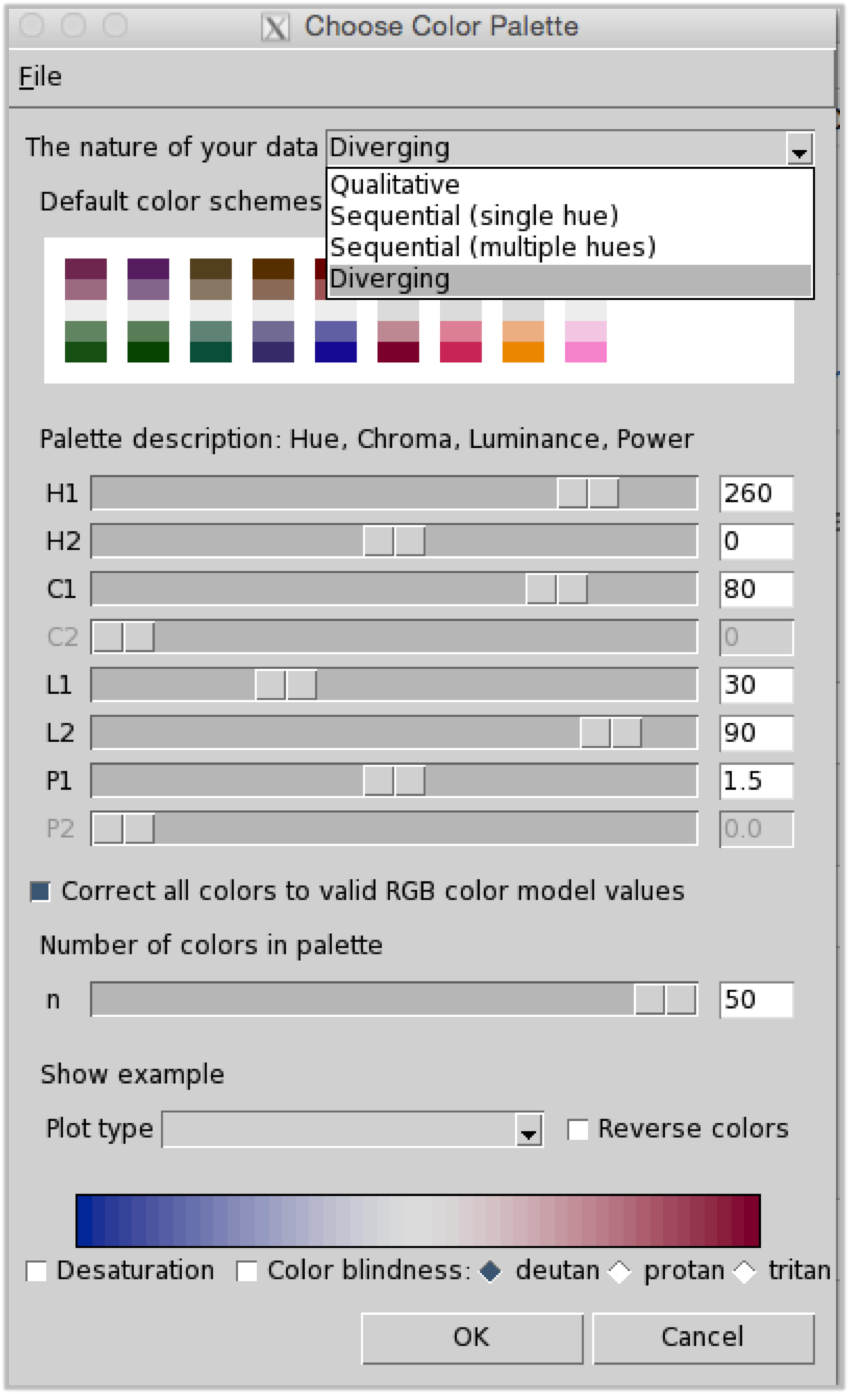
\includegraphics[scale=.4]{figures/ss_colorscheme.png}
\end{center}

The bar at the bottom will reflect your choices and should give you a good idea of how your plot will be affected. In addition, you can choose to see an example plot, e.g. a pie chart.
Note that this example will not be shown within the app, but in RStudio's \textsf{Plot} environment!
\begin{center}
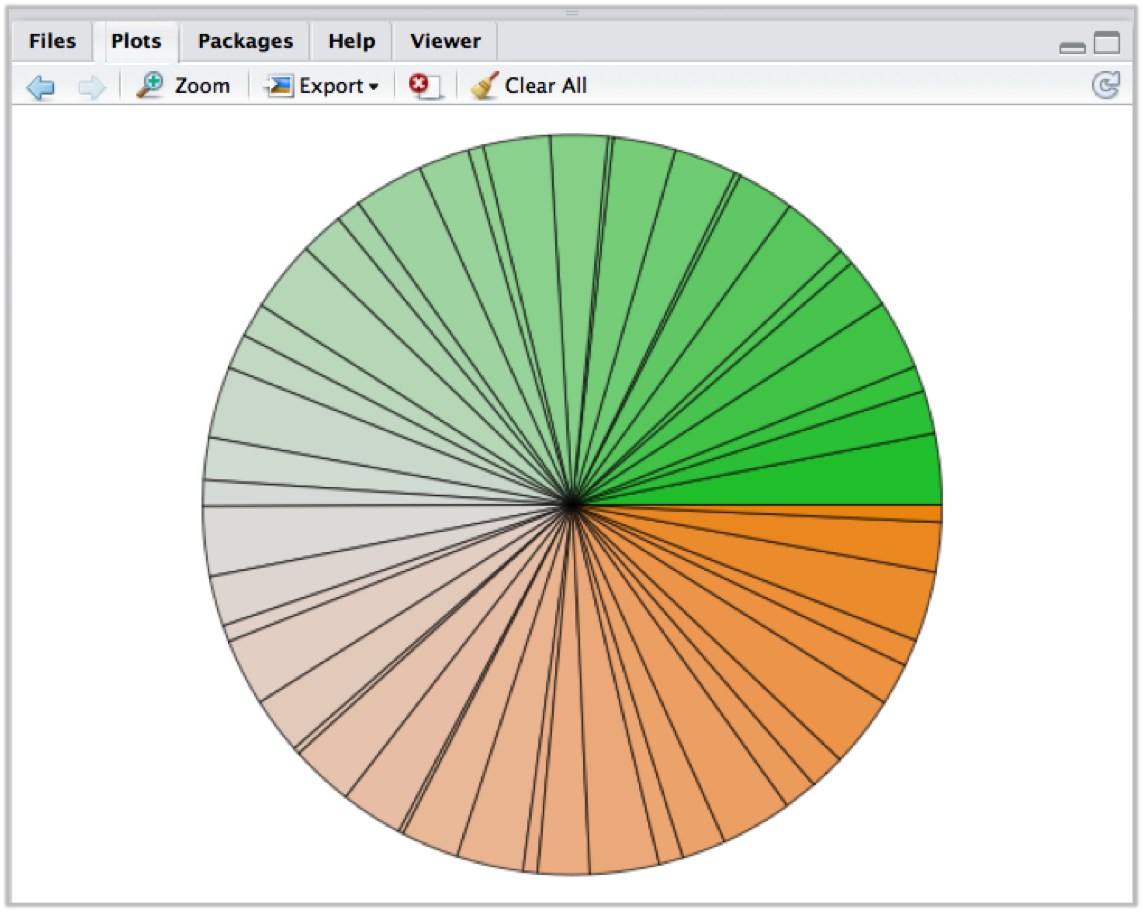
\includegraphics[width=.95\columnwidth]{figures/ss_colorscheme_example.png}
\end{center}

%---------------------------------------
\subsection{Summary plots}
%---------------------------------------

Summary plots display the sum of all measurements per fraction.
The default setting will make one plot per selected experiment ID.
If you would like to visually distinguish the different fractions, choose a different color scheme.

\begin{center}
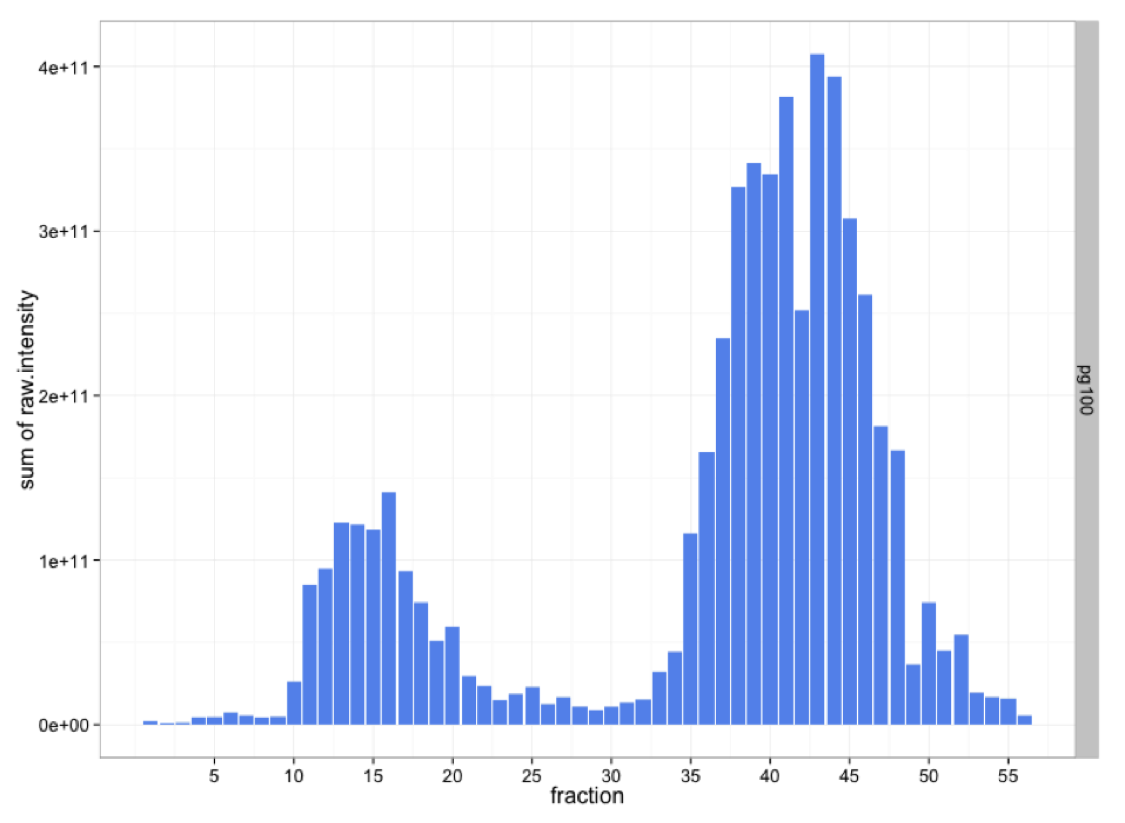
\includegraphics[scale=.4]{figures/ss_sumPlot_example.png}
\end{center}

\bangbox{Since the summary plots will have to retrieve and compute \textit{all} values per experiment, the generation of the image may take a couple of seconds.}

%---------------------------------------
\subsection{Individual proteins}
%---------------------------------------

The individual protein plots are useful to track the measurements for single protein across the different fractions.

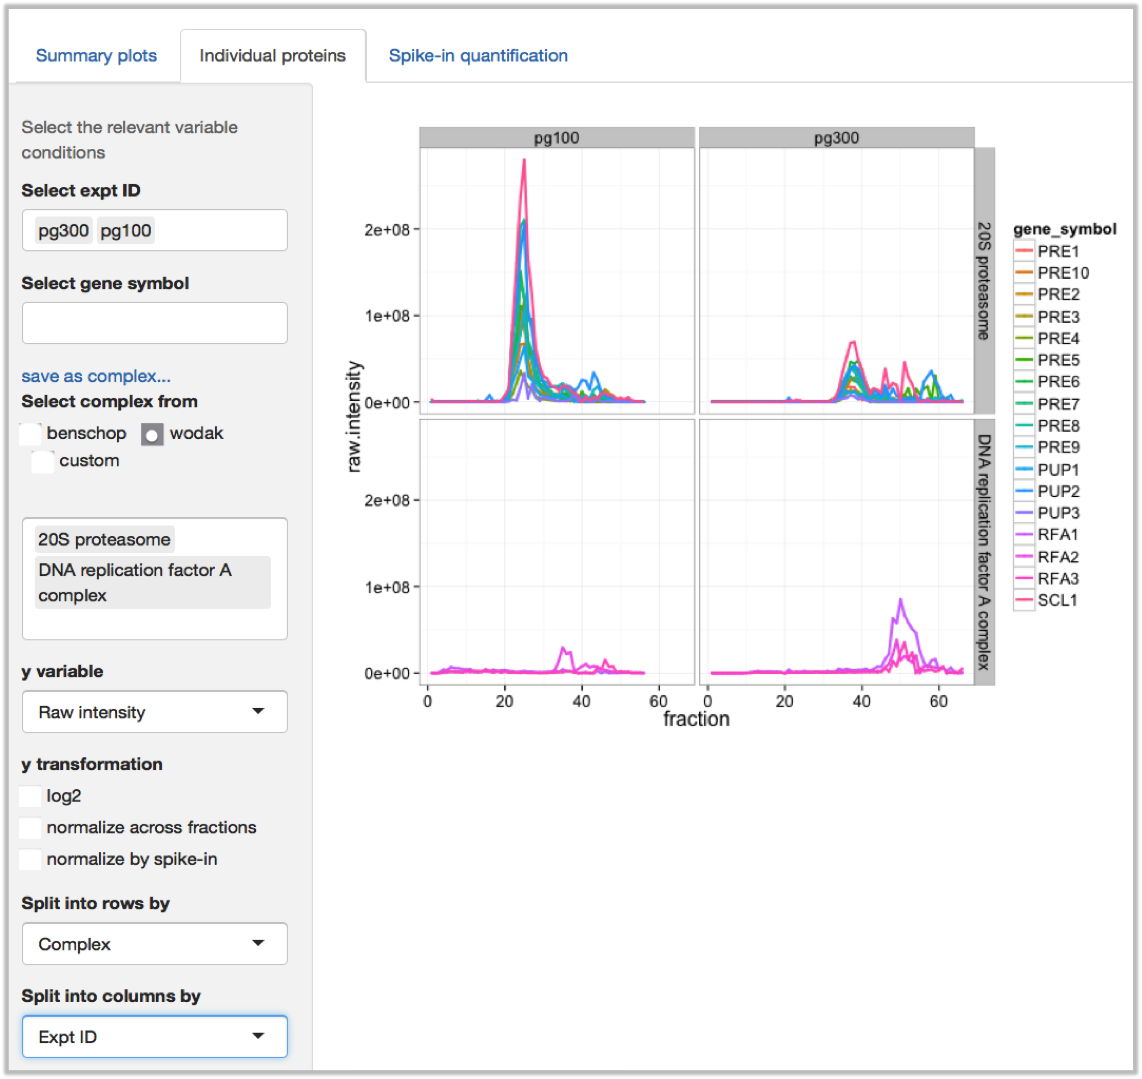
\includegraphics[width=\columnwidth]{figures/ss_indProt_example.png}

As for the summary plots, start by \textit{selecting the experiment ID(s)}. Once you have selected the first experiment ID, the list of possible additional experiment IDs will be reduced based on the organism of your first selection. This way, you will always only be able to compare samples from the same organism. This also means that you should wait for the successful loading of the first data set which will be indicated by a message stating the organism of your choice.

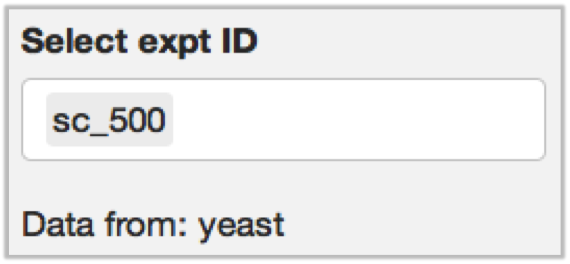
\includegraphics[width=.5\columnwidth]{figures/ss_indProt_start.png}

To display protein profiles of interest, select them by their gene name or their UniProt ID, e.g. "GAPDH".

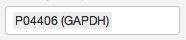
\includegraphics[width=.5\columnwidth]{figures/ss_uniprot_entry.png}


\paragraph*{Customizing the plots}
There are numerous options to customize the display to allow for useful comparisons, e.g., across experiments and between the members of distinct protein complexes.

Typically, it will make sense to \textit{assign the color based on the gene symbol}.
The legend will always be sorted alphabetically, and so will the table of basic information that you can retrieve from UniProt.

To compare multiple complexes across different experiments, we recommend to \textit{split by rows} using the experiment IDs and to \textit{split by columns} using the complex' IDs.

You can also choose to differentiate different gene symbols by the point shape or line type, but note that this makes only sense for very limited numbers of variables (up to 5 different genes, for example).

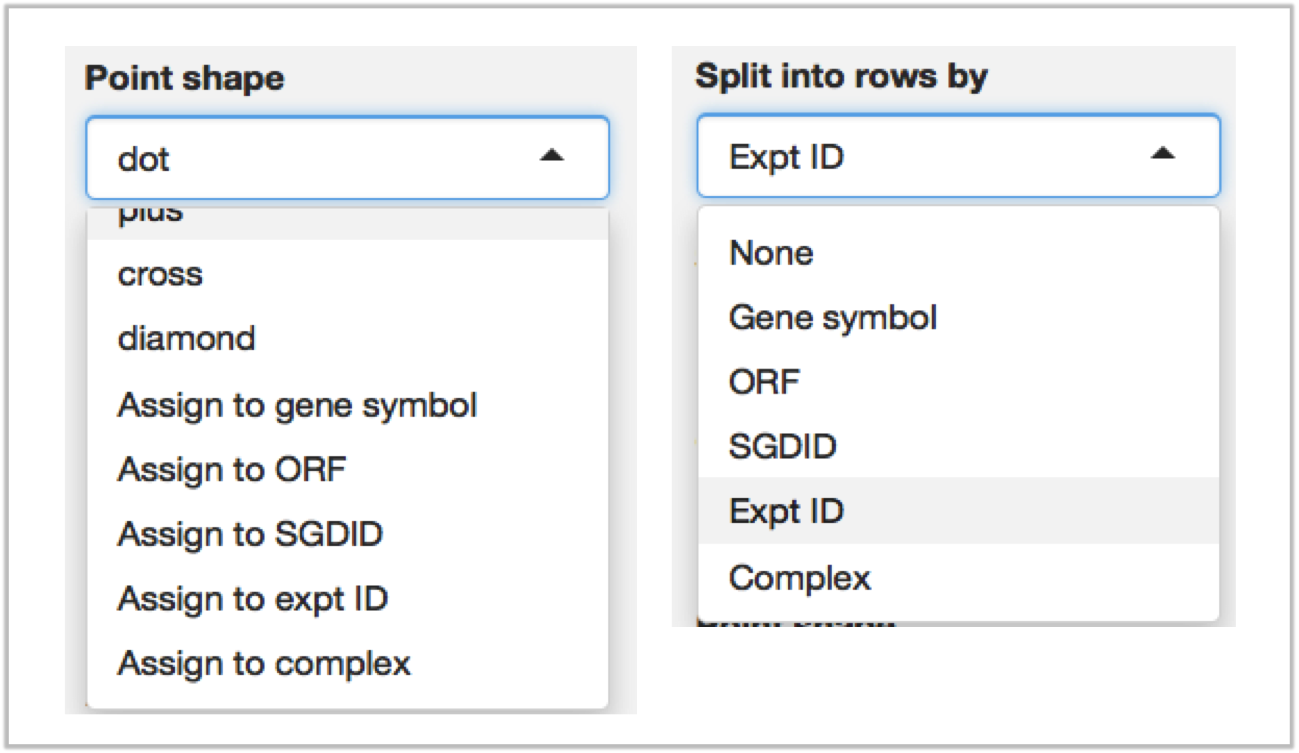
\includegraphics[width=\columnwidth]{figures/ss_plotOptions.png}

If you have replicates for the same experimental condition, you can specify both, the name of the condition and numeric replicate labels.
For this, you will have to check the box \textsf{Specify replicates} underneath the box for the selection of the experiment IDs.
You can then manually define the name of the experimental condition, which can then be used  to, for example, split the plots.

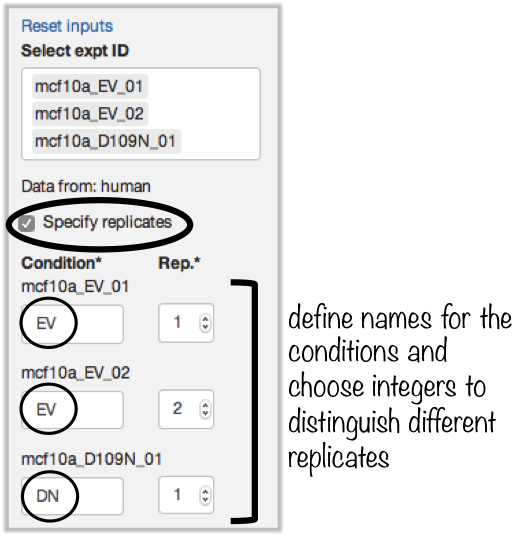
\includegraphics[width=\columnwidth]{figures/ss_plotCustomizing02.png}

A useful combination of settings may be:
\begin{itemize}[noitemsep]
\item \textsf{Split into rows by:} Gene symbol
\item \textsf{Split into columns by:} Condition
\item \textsf{Color by:} Replicate
\end{itemize}

This would result in the following figure:

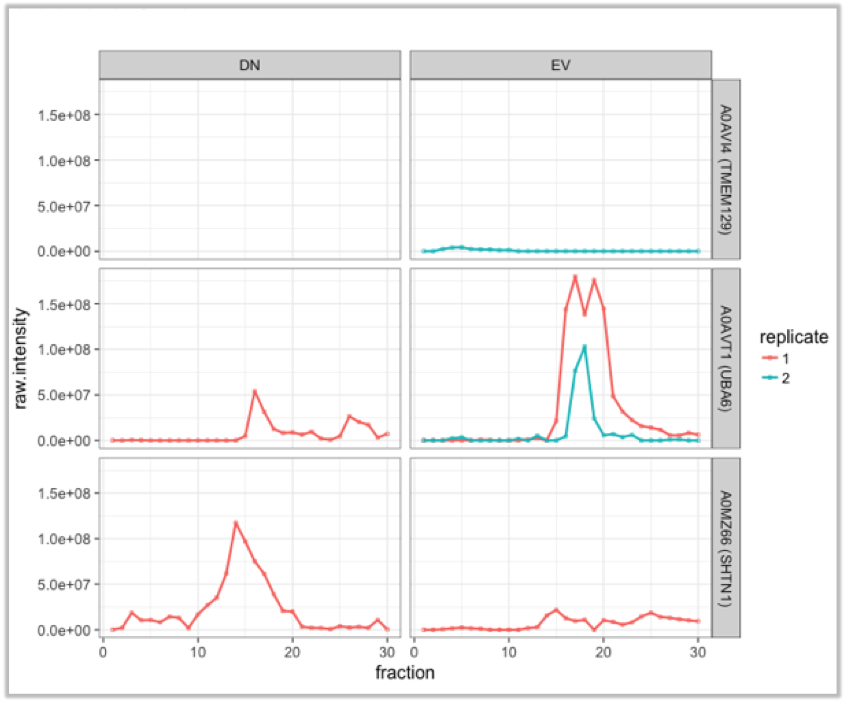
\includegraphics[width=\columnwidth]{figures/ss_plotCustomizing03.png}

\paragraph*{Normalization} The values displayed on the y-axis can be $log$-transformed or normalized using two approaches: either across fractions or by using a spike-in control.
When normalizing based on the values for spike-in controls, you will be able to choose the specific protein if more than one standard was indicated in the metadata section for any experiment.

\begin{center}
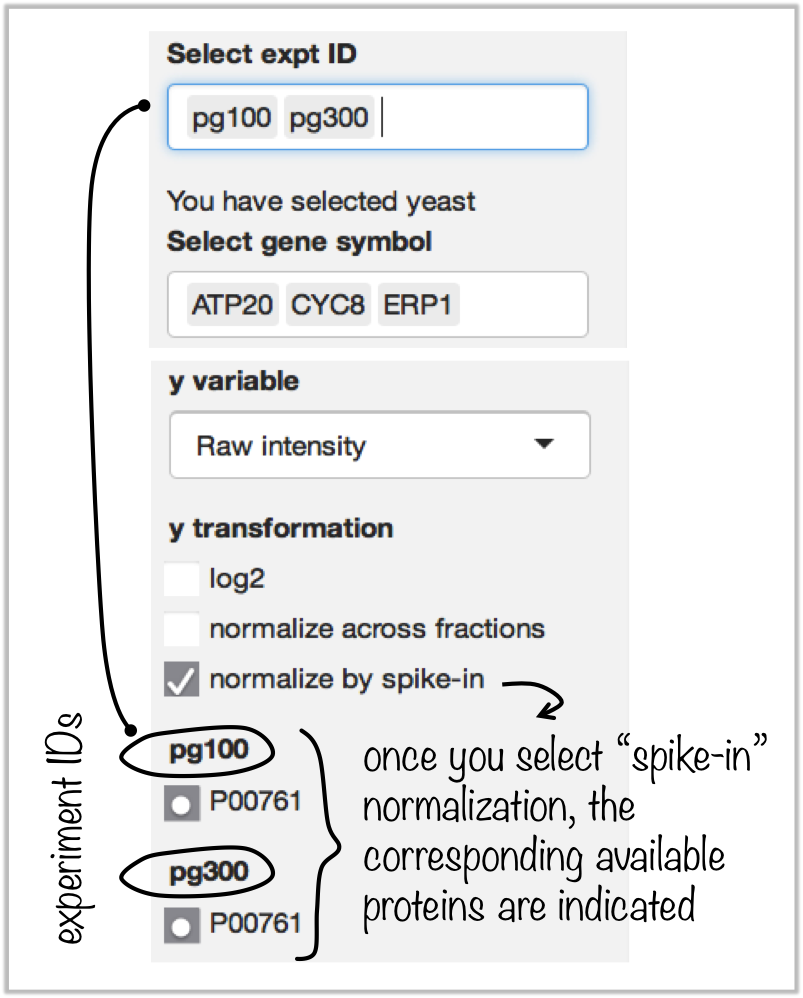
\includegraphics[width=.8\columnwidth]{figures/ss_indProt_normSpikeIn.png}
\end{center}

For details on the normalization of the y variable, see Section \ref{sec:norm}.

\paragraph*{Complexes} Instead of specifying individual gene symbols that should be displayed, you can also select a set of proteins that have been reported to be part of common complexes.
We currently supply three lists of complexes: two for yeast based on publications by Benschop et al. \citep{Benschop2010}, and Wodak et al. \citep{Wodak2009}, and one for human complexes, \textsf{CORUM Core} \citep{corum}.

To see the profiles for proteins of a complex defined by either one, e.g., select \textsf{``Wodak"}, then use the empty field below to search for the complex of interest, e.g. \textsf{``20S Proteasome"}.
You can select multiple protein complexes.
To add additional proteins, use the field \textsf{``Select gene symbol"}.


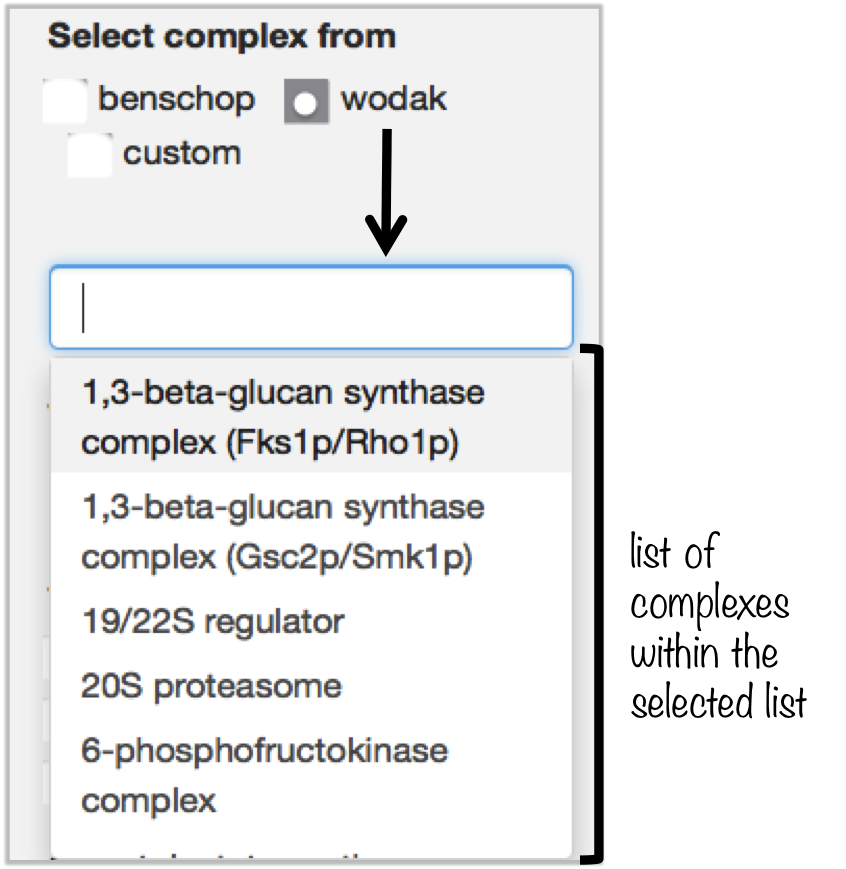
\includegraphics[width=.7\columnwidth]{figures/ss_complexes01.png}

\bangbox{Many complexes may encompass proteins for which your experiment does not provide any values. This will cause \textsf{NA} entries.}

If you want to limit the complexes that are available in the auto-select box to those for which many proteins were recovered in your experiment(s), you can specify the minimum number of proteins per complex that should be present in \textit{every} experiment.

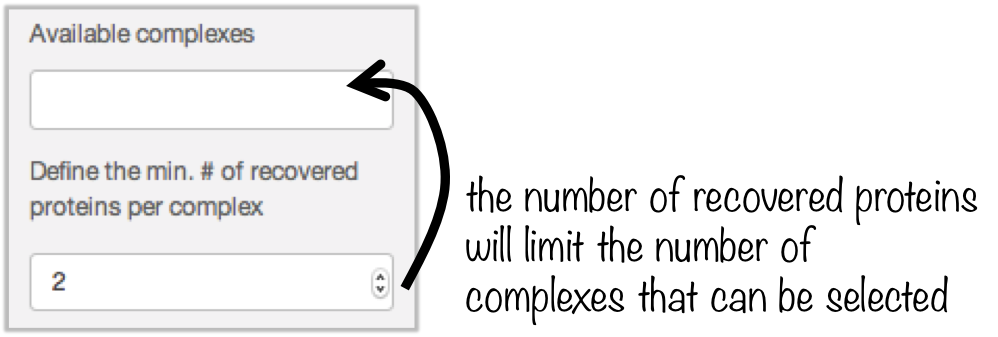
\includegraphics[width=.9\columnwidth]{figures/ss_complexes02.png}

In addition to the pre-defined complexes, you can \textit{generate your own groups of proteins}.
Simply choose the individual proteins that you would like to group together via the \textsf{``Select gene symbol"} line, then hit \textsf{``save as complex..."}.
You will be asked to specify a name for the protein group.
Once you have saved a group, it will be available in all future sessions: simply select the \textsf{``custom"} field and use the empty line below to select your custom-made group of interest.



%---------------------------------------
\subsection{Spike-in quantification}
%---------------------------------------

Ideally, each experimental ID should have the corresponding UniProt ID for the spike-in protein that was used.
Therefore, all you will have to do here is to indicate the experiment(s) of interest and the profiles for the spike-ins related to the experiment(s) will be shown.

If no UniProt ID was specified during the upload of the file (as described in Section \ref{sec:dataup}), Trypsin from pig (UniProt ID P00761) will be used.

\begin{center}
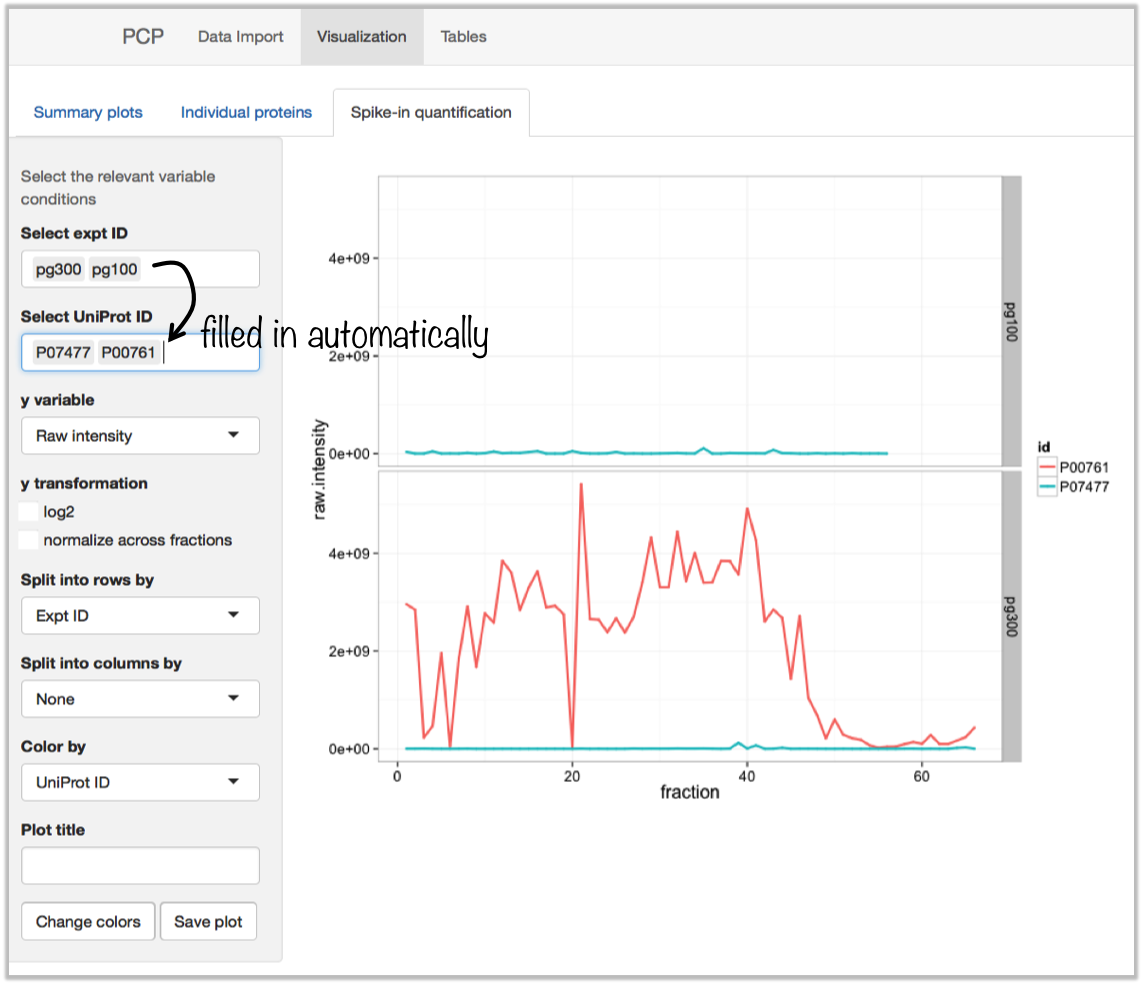
\includegraphics[width=.98\columnwidth]{figures/ss_spikeIn01.png}
\end{center}

The field \textsf{``Select UniProt ID"} will be automatically populated depending on the experiment ID. You can delete individual entries, but you cannot add spike-ins. Use the \textsf{``Individual proteins"} plots for assessing individual protein profiles.

%===================
\section{Tables}
%===================


\includegraphics[scale=.5]{figures/ss_appOverview03.png}

The tables section allows you to see the values that underlie the summary plots and individual protein profiles.
Conversely, if the visualization section is empty (e.g., because you haven't selected an experimental ID), the corresponding table section will be empty, too.
The following example shows the table for the summary plot.

\begin{center}
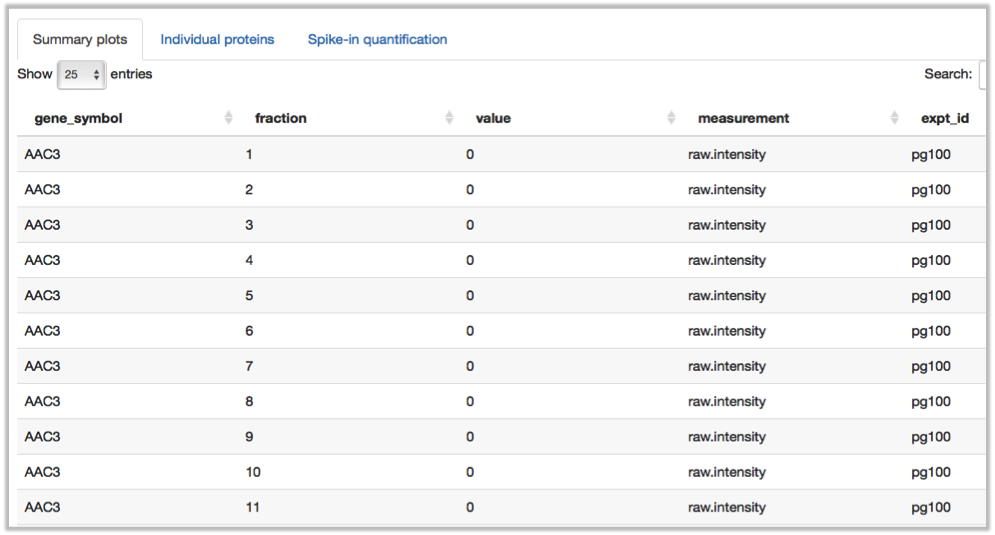
\includegraphics[width=.99\columnwidth]{figures/ss_table01.png}
\end{center}

Each row corresponds to \emph{one} fraction per protein per experiment ID, which is different from \texttt{MaxQuant}'s table where each row corresponds to \textit{all} fractions per protein and experiment ID. 

%========================
\section{Correlations}
%========================



\includegraphics[width=\columnwidth]{figures/ss_appOverview05.png}

Define Condition (\textsf{Cond}) and replicate numbers (\textsf{Repl.}) that correspond to the experimental ID.

%Calculating may take a while.
%``Smoothed" means Friedman's superSmoother.
%What is the correlation based on? Covariance?

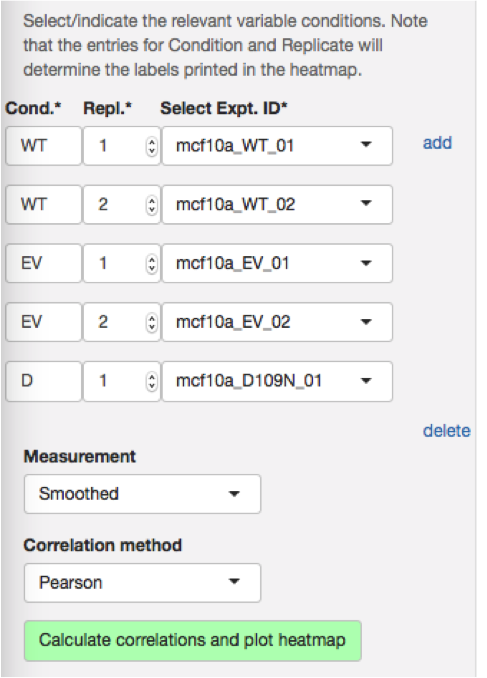
\includegraphics[width=\columnwidth]{figures/ss_correlations01.png}

%Explain Pairwise vs. Conditionwise and Subset

Currently saving has to be done via right-mouse click


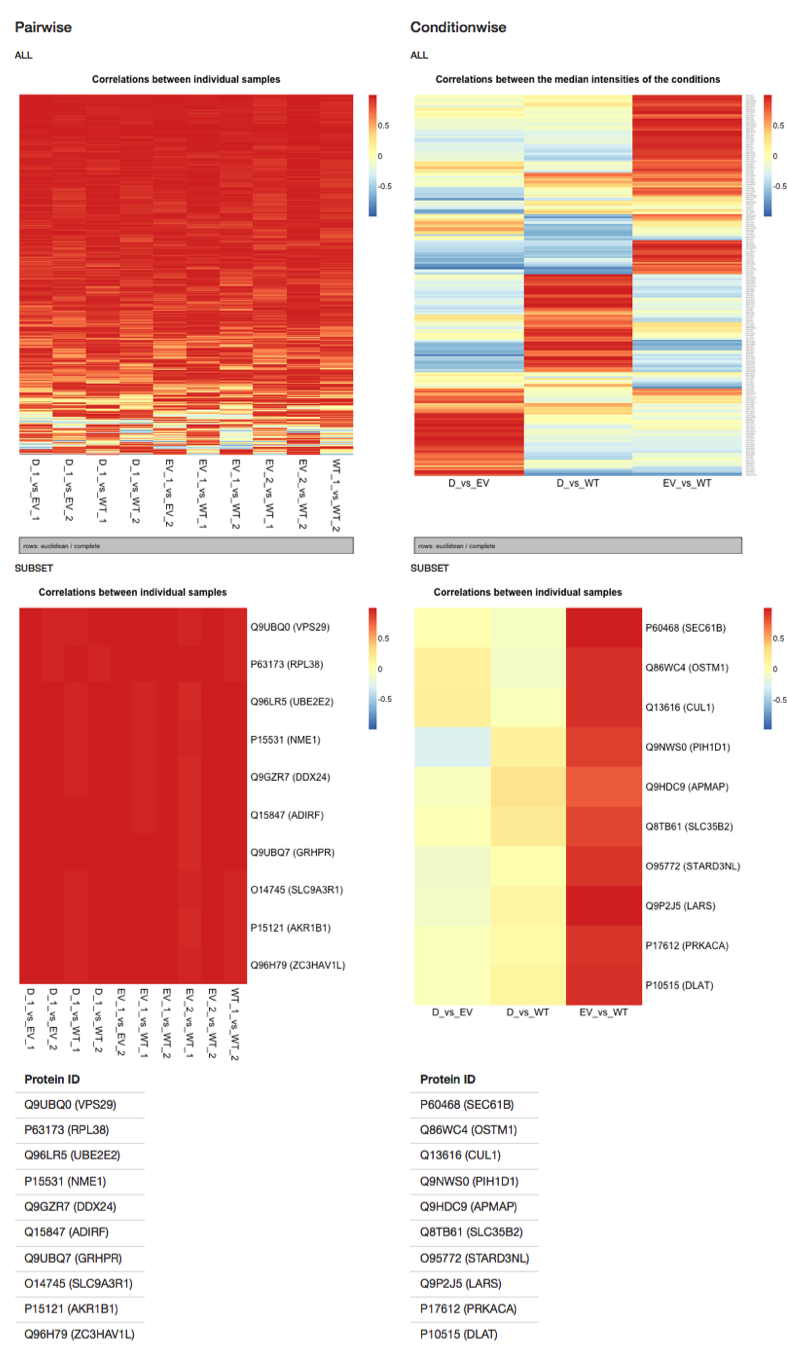
\includegraphics[width=\columnwidth]{figures/ss_correlations_hm.png}

%-------------------------------------------------------
\subsection{Reducing the numbers of displayed proteins}
%-------------------------------------------------------

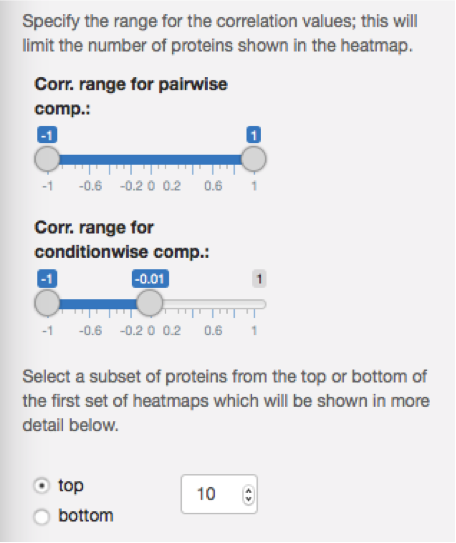
\includegraphics[width=\columnwidth]{figures/ss_correlations02.png}

Limit the range of correlation values

specify the number of proteins shown in the subsets


%-------------------------------------------------------
\subsection{Defining proteins of interest for protein profile plots}
%-------------------------------------------------------

%Explain the route via pre-defined complexes

\clearpage
\onecolumn
\bibliographystyle{../../ABCreference}
\setlength{\bibsep}{2pt}
\bibliography{references_PCP}

\end{document}
